\documentclass{beamer}
\usetheme{Boadilla}
\usepackage[utf8]{inputenc}
\usepackage{booktabs}
\usepackage{threeparttablex}
\usepackage{mathpazo}
\usepackage[mathpazo]{flexisym}
\usepackage{array}
\usepackage{caption}
\captionsetup[figure]{font=scriptsize}
\usepackage{graphicx}
\usepackage{threeparttablex}
\usepackage[labelformat=empty]{subfig}
\usepackage[T1]{fontenc}
\usepackage{tikz}

\newcommand\hd[2]{\multicolumn{2}{c}{\begin{tabular}{@{}c@{}}#2\end{tabular}}}
\newcolumntype{C}[1]{>{\centering\let\newline\\\arraybackslash\hspace{0pt}}m{#1}}
\let\estinput=\input
\newcommand{\estwide}[3]{
        \vspace{.75ex}{
            \textsymbols
            \begin{tabular*}
            {\textwidth}{@{\hskip\tabcolsep\extracolsep\fill}l*{#2}{#3}}
            \toprule
            \estinput{#1}
            \bottomrule
            \addlinespace[.75ex]
            \end{tabular*}
            }
        }

\newcommand{\estauto}[3]{
        \vspace{.75ex}{
            \textsymbols
            \begin{tabular}{l*{#2}{#3}}
            \toprule
            \estinput{#1}
            \bottomrule
            \addlinespace[.75ex]
            \end{tabular}
            }
        }

\newcommand{\specialcell}[2][c]{%
    \begin{tabular}[#1]{@{}c@{}}#2\end{tabular}
}

\definecolor{MyBackground}{rgb}{0.95,0.95,0.96}
\setbeamercolor{background canvas}{bg=MyBackground}

\definecolor{UniBlue}{RGB}{83,121,170}
\setbeamercolor{title}{fg=UniBlue}
\setbeamercolor{frametitle}{fg=UniBlue}
\setbeamercolor{structure}{fg=UniBlue}
\setbeamertemplate{footline}{}

\AtBeginSection[]{
  \begin{frame}
  \vfill
  \centering
  \begin{beamercolorbox}[sep=8pt,center,shadow=true,rounded=true]{title}
    \usebeamerfont{title}\insertsectionhead\par%
  \end{beamercolorbox}
  \vfill
  \end{frame}
}

\title[]{Publishing in Economics}
\date{}

\begin{document}

\maketitle

\beamertemplatenavigationsymbolsempty
\begin{frame}{Publishing in Economics - Process}
    \begin{itemize}
        \item Kitt Carpenter - \color{blue} \href{https://www.appam.org/how-many-journals-work-a-far-from-incomplete-guide-for-public-policyeconomics-scholars/?pg=58&F_All=y}{How (many) journals work}
    \end{itemize}
    \bigskip
    \begin{itemize}
        \pause \item \textbf{Step 1: Pre-review check} 
        \begin{itemize}
            \item Primarily formatting.
        \end{itemize}
        \medskip
        \pause \item \textbf{Step 2: Managing editor review}
        \begin{itemize}
            \item ``Broad skim of paper for fit and quality'' (does not read entire paper).
            \begin{itemize}
                \item[-] Is this research interesting, novel, and important?
                \item[-] Is this research likely of interest to readers of the journal?
                \item[-] Does the paper appear competently communicated and executed?
            \end{itemize}
            \item Desk rejection phase.
            \item Timing: 2 weeks to 2 months.
        \end{itemize}
    \end{itemize}          
\end{frame}

\begin{frame}{Publishing in Economics - Process}
\begin{itemize}
    \item \textbf{Step 3: Co-editor check}
    \begin{itemize}
        \item Managing editor assigns paper to a co-editor (\color{blue} \href{https://www.aeaweb.org/journals/aer/about-aer/editors}{example}\color{black}).
        \item Co-editor is an expert in the paper's field (usually reads entire paper).
        \item Identifies reviewers and sends paper out for review.
        \item Can still desk reject.
        \item Timing: 2 to 6 months.
    \end{itemize}
\medskip
    \pause \item \textbf{Step 4: Final decision}
    \begin{itemize}
        \item Co-editor evaluates reviewer comments (and their own thoughts on the paper). 
        \item Makes an accept/revise/reject decision or recommendation to the managing editor.
    \end{itemize}
\end{itemize}
\end{frame}

\begin{frame}{Publishing in Economics - Sample Rates}
    \begin{figure}
        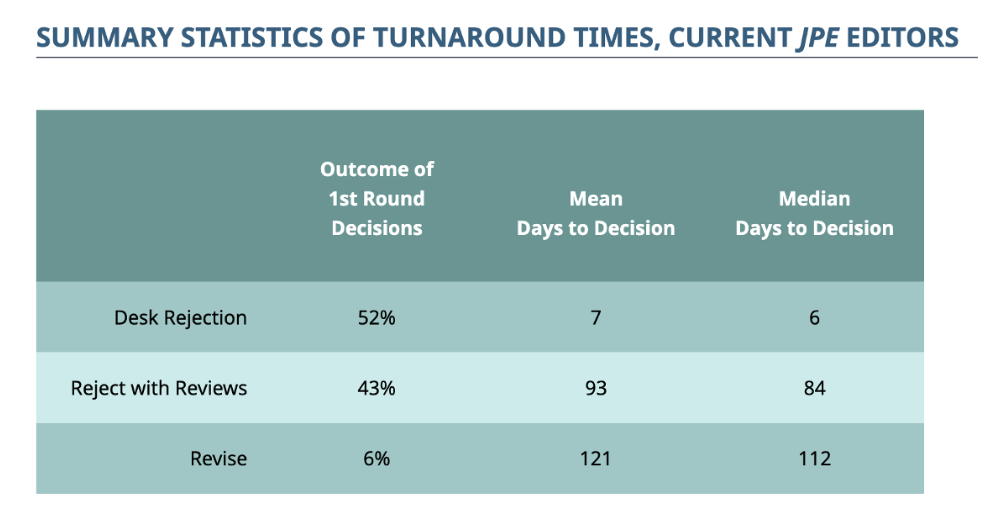
\includegraphics[scale=0.55]{images/jpe.png}
    \end{figure}      
\end{frame}

\begin{frame}{Publishing in Economics - Sample Rates}
    \begin{figure}
        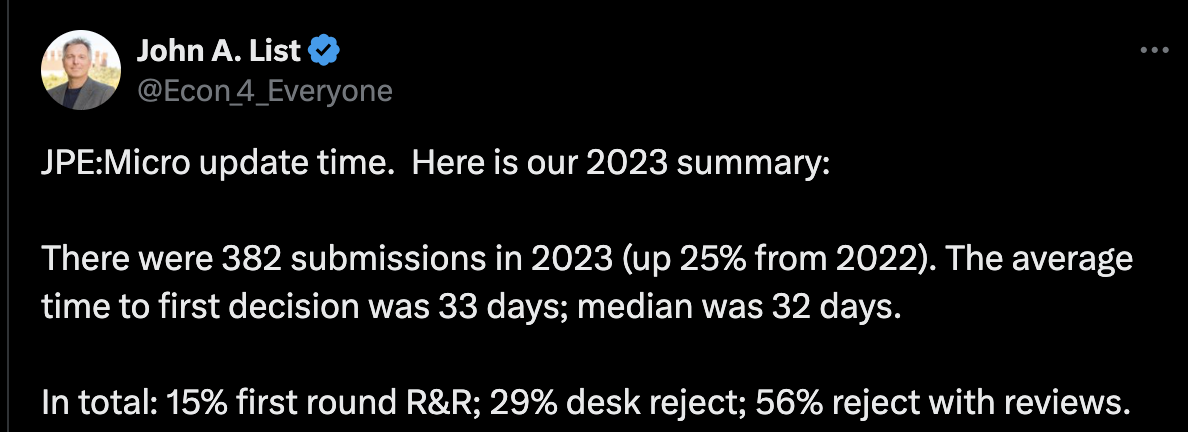
\includegraphics[scale=0.45]{images/jpe_micro.png}
    \end{figure}      
\end{frame}

\begin{frame}{Publishing in Economics - Sample Rates}
    \begin{figure}
        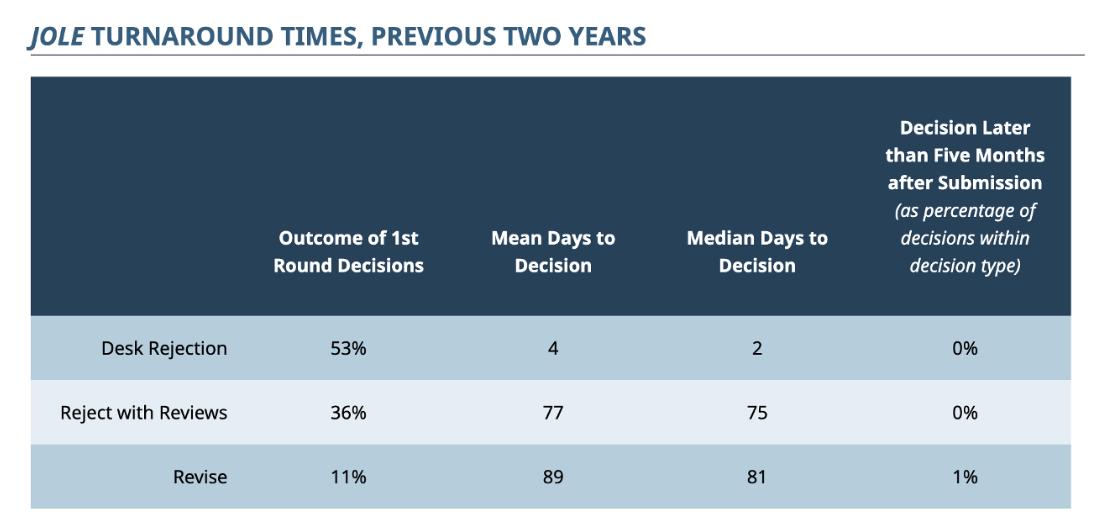
\includegraphics[scale=0.55]{images/jole.png}
    \end{figure}      
\end{frame}

\begin{frame}{Publishing in Economics - Kitt's tips}
    \begin{itemize}
        \item \textbf{How important to meet style guide?}
        \begin{itemize}
            \item Meet word/page count other stuff less important.
        \end{itemize}
        \smallskip
        \pause \item \textbf{How much to revise?}
        \begin{itemize}
            \item Desk reject - may not need revision, target lower journal.
            \item Reviewer reject - address reasonable comments (you may get the same reviewer).
            \item Revise and resubmit - do everything the reviewers ask you to do (not all may make the paper).
        \end{itemize}
        \smallskip
        \pause \item \textbf{When is it ok to contact the editor about paper status?}
        \begin{itemize}
            \item 3 to 6 months after submission.
        \end{itemize}
        \smallskip
        \pause \item \textbf{When is it ok to appeal an editor's decison?}
        \begin{itemize}
            \item Almost never.
            \item Did a reviewer make a factual error and did the editor state this as a reason for rejection?
        \end{itemize}
    \end{itemize}
\end{frame}

\begin{frame}{Publishing in Economics - Kitt's tips}
    \begin{itemize}
        \item \textbf{How to not get desk rejected?}
        \begin{itemize}
            \item Write well (this is my tip!).
            \item Make sure your paper is a good fit for the journal.
            \begin{itemize}
                \item[-] Signal fit in your cover letter.
                \item[-] Cite papers from the journal.
            \end{itemize}
        \end{itemize}
        \medskip
        \pause \item \textbf{Most common mistake?}
        \begin{itemize}
            \item Me: “Where will you send this paper?”  
            \item Junior Colleague: “Journal A, B, or C”.  
            \item Me: “Who would likely handle the paper at each of those journals?”  
            \item Junior Colleague: “I don’t know”. 
        \end{itemize}
    \end{itemize}
\end{frame}

\begin{frame}{Submission checklist}
    \begin{itemize}
        \item \color{blue} \href{https://docs.google.com/document/d/1JwwmOgRhd2p-Bl_RFEMnp04P0I2nNhOHW7JHdaLcyGs/edit}{Mirya Holman's pre-submission checklist}
    \end{itemize}
\end{frame}

\end{document}